% Supplementary material for "Governing Societies of AI Agents".
% Standalone: compiles on its own and shares no labels with the manuscript.
\documentclass[11pt,a4paper]{article}
\usepackage[margin=1in]{geometry}
\usepackage[T1]{fontenc}
\usepackage{lmodern}
\usepackage{microtype}
\usepackage{parskip}
\usepackage{booktabs}
\usepackage{longtable}
\usepackage{enumitem}
\usepackage{graphicx}
\usepackage{amsmath}
\usepackage{amssymb}
\usepackage{natbib}
\bibliographystyle{plainnat}
\usepackage[hidelinks]{hyperref}

\title{\vspace{-2em}\textbf{Supplementary Material}\\[0.3em]
\large Governing Societies of AI Agents: Committed Minorities,\\
Model Diversity, and Scale as Levers of Multi-Agent AI Governance}
\author{Gopal Kalyanaraman \and Vijay K.\ Madisetti}
\date{}

\begin{document}
\maketitle
\vspace{-1.5em}

\noindent
This supplement holds material that supports but is not central to the argument of
the main paper: a self-contained mechanical study of institutional decision rules,
the full institutional-ladder arms, the granularity account of commons survival,
the sustainability--equity trade-off, a methodological caution about token budgets
in scale studies, and supporting figures and mappings whose values are stated in
the main text. Every figure and table here is generated from the released result
files at \url{https://github.com/kalyanar/governing-societies-of-ai-agents}.

\bigskip\hrule\bigskip



Material supporting but not central to the argument: a mechanical study of
decision rules, the full institutional-ladder arms, the granularity account of
commons survival, the sustainability--equity trade-off, a caution about token
budgets in scale studies, and supporting figures and mappings.

\subsection*{C.1 Institutional rules set the capture threshold}
The capture threshold is not an intrinsic property of a society; rather, it is determined by the operative decision rule. In a Granovetter-style cascade framework—where a committed subset of advocates promotes a change against an established status quo, free agents adopt the change once observed assembly support exceeds their individual adoption thresholds, and the system is initialized with $400$ seeds—the fraction of committed minority agents required to \emph{capture} the collective decision is highly sensitive to the institutional rule (see the institutional-rules figure in Appendix~A of the main paper). Under simple majority rule, capture occurs at approximately $p_c \approx 30\%$. A $2/3$ supermajority rule increases resistance to capture, raising the threshold to roughly $37.5\%$. By contrast, \emph{delegation} (liquid democracy, in which free agents delegate their vote to the advocate bloc) dramatically reduces the effective capture threshold to about $7.5\%$. A \emph{veto} or consensus rule allows a single committed defender (approximately $1.7\%$ of the assembly) to capture the decision by persistent obstruction.

An LLM council–style confirmation setting ($N{=}7$, with gpt-4o-mini and Claude-Haiku monocultures versus a mixed council, initialized with $5$ seeds) introduces an important qualification: sufficiently capable councils \emph{do not become persuaded} by the reckless proposal. Free members systematically reject the unsafe option regardless of the number of advocates, implying that capture only occurs when the advocate bloc alone is large enough to mechanically satisfy the decision rule, and that a supermajority requirement prevents capture even in this case. In this regime, homogeneous and heterogeneous councils exhibit essentially identical behavior, because each individual member is sufficiently competent to converge independently on the prudent decision. This is consistent with the main text, where council composition influenced open-ended \emph{stance diversity} but had negligible effect on decisions for which there is a clearly prudent alternative. The aggregation rule is one institutional lever; the \emph{enforcement} mechanism is another---\citet{bell2026restitution} show that restitution (returning a sanctioned agent's gains) contains a defecting minority where deterrence alone fails, complementary to the voting rules studied here.

\emph{Governance implication:} the choice of decision rule must be made deliberately. Supermajority requirements increase resistance to capture (at the expense of reinforcing the status quo), whereas delegation and veto-style rules create powerful capture channels for a very small, committed minority.

\subsection*{C.2 Institutional ladder: full arms}
\paragraph{Each institutional layer buys tolerance of one more defector.}
Blindness and self-interest are design choices, not properties of LLM agents, and
Ostrom's field studies of durable human commons identify precisely what they omit:
mutual monitoring and graduated sanctions~\cite{ostrom1990}. We therefore add
them one at a time (the table below), holding the world model fixed.
\emph{Monitoring} reveals each agent's catch from the previous month.
\emph{Stewardship} replaces the self-interested objective with one directed at the
resource persisting and the catch being shared fairly. \emph{Restitution} returns
an over-harvester's excess to the resource before regeneration.

\begin{table}[t]
\caption{Institutional layers, $N{=}5$, $30$-month horizon, 3 seeds per cell.
Every cell is clean ($0/3995$ decisions defaulted across all arms).}
\label{tab:arms}
\small
\begin{tabular}{@{}p{5.4cm}cccc@{}}
\toprule
\textbf{Society} & \textbf{0 def.} & \textbf{1 (20\%)} & \textbf{2 (40\%)} & \textbf{3 (60\%)} \\
\midrule
Blind, self-interested & holds & dies $16$--$28$ & dies $6$--$7$ & --- \\
Monitored, self-interested & holds & dies $10$--$12$ & dies $4$--$7$ & --- \\
Monitored, \emph{steward} & holds & \textbf{holds} & dies $8$--$12$ & --- \\
\;\;+ \emph{restitution} & holds & holds & \textbf{holds} & \textbf{holds} \\
\bottomrule
\end{tabular}
\end{table}

Two results stand out. First, \emph{monitoring alone is mildly harmful}: making
defection visible without any means of redress accelerates collapse from
$16$--$28$ months to $10$--$12$. Information is not a governance control. Second,
the objective is the first lever that works. Given the compensatory catch of
the collapse-time law---$6.0$ tons at a stock of $80$ with one defector---steward
agents select exactly $6.0$ where self-interested agents select their fair share
of $8.0$. Adding restitution extends tolerance to three defectors in five while
retaining $80$--$92\%$ of the adversary-free yield. A steward society therefore
does possess a genuine capture threshold, bracketed by our measurements between
$20\%$ (absorbed indefinitely) and $40\%$ (collapse within $8$--$12$ months);
with restitution the bracket moves to between $60\%$ and $80\%$. At $N{=}5$ these
brackets are one defector wide and we do not claim a point estimate inside them.

\subsection*{C.3 Token budget confounds scale}
\paragraph{Token budget confounds scale.} A methodological caution for anyone
running such probes: reasoning-tuned models must be given room to finish. Measured
at a $150$--$500$ token cap, our $24$--$31$B candidates scored $0.21$--$0.38$;
re-measured at $2{,}500$ tokens with an otherwise identical prompt, the same models
scored $0.71$--$1.00$ with a $1.00$ parse rate throughout. The entire apparent
deficit was truncation before the answer marker. Scale studies that hold
\texttt{max\_tokens} fixed across a generation boundary will therefore report a
capability curve that is partly an artifact of the budget.

\subsection*{C.4 Absolute restraint versus adversary share}
\paragraph{The governing quantity is absolute restraint, not adversary share.}
The committed-minority fraction does not organize these results. A society of five
survives one defector ($20\%$) while a society of ten dies at two ($20\%$); a
$40\%$ minority is survivable with restitution and fatal without; $60\%$ is
survivable where $80\%$ is not. Sorting instead by the per-agent catch that
the collapse-time law demands separates every observed outcome without exception
(the table below): each of the seven configurations requiring more than
$4.4$ tons survives, and each of the five requiring less than $3.8$ dies. The
boundary is an absolute quantity, and it coincides with the granularity at which
these agents express a decision---they answer in whole and half tons, so a target
of $2.5$ or $3.3$ tons is one they cannot reliably hit, while $7.5$ is.

\begin{table}[t]
\caption{Every steward configuration measured, ordered by the restraint
the collapse-time law requires. Survival tracks the absolute catch, not the
adversary share.}
\label{tab:absolute}
\small
\begin{tabular}{@{}ccccr@{}}
\toprule
$N$ & \textbf{def.} & \textbf{share} & \textbf{restitution} & \textbf{required catch $\to$ outcome} \\
\midrule
5  & 0 & 0\%  & --        & $10.00$ \;holds \\
5  & 1 & 20\% & \checkmark & $9.50$ \;holds \\
5  & 2 & 40\% & \checkmark & $8.67$ \;holds \\
5  & 1 & 20\% & --        & $7.50$ \;holds \\
5  & 3 & 60\% & \checkmark & $7.00$ \;holds \\
10 & 1 & 10\% & --        & $4.44$ \;holds \\
\midrule
10 & 2 & 20\% & --        & $3.75$ \;dies \\
5  & 2 & 40\% & --        & $3.33$ \;dies \\
10 & 3 & 30\% & --        & $2.86$ \;dies \\
5  & 4 & 80\% & \checkmark & $2.00$ \;dies \\
10 & 4 & 40\% & --        & $1.67$ \;dies \\
\bottomrule
\end{tabular}
\end{table}

This also explains the effect of scale. Because the required catch falls as $1/N$,
a twenty-agent society must hold each member to $2.5$ tons even with no adversary
present---below the expressible floor---and it collapses within $4$--$6$ months at
$p=0$. Group size, defector count and enforcement are not independent risks; they
trade against one another on the single axis of how much restraint each agent must
articulate.

\emph{Governance interpretation:} the tolerable committed minority is a property
of institutional design rather than of the agent population, ranging in our
measurements from none at all (blind, self-interested) to three in five (steward
with restitution). A share cap is therefore the wrong control here---the defence
our opinion-dynamics results in the main text motivate does not transfer.
What transfers is Ostrom's pairing: an objective that makes the resource's
persistence the agent's own aim, and an enforcement rule that reclaims what a
defector takes, which is the mechanism \citet{bell2026restitution} find necessary
where informal pressure fails. Our monitoring-only arm shows why informal pressure
is insufficient. A third lever is specific to artificial agents and has no direct
analogue in Ostrom's field settings: because the binding constraint is the
granularity at which restraint can be expressed, widening the action space---%
permitting fractional allocations rather than whole units---should raise
tolerance without changing the institution at all.

\begin{figure}[t]
\centering
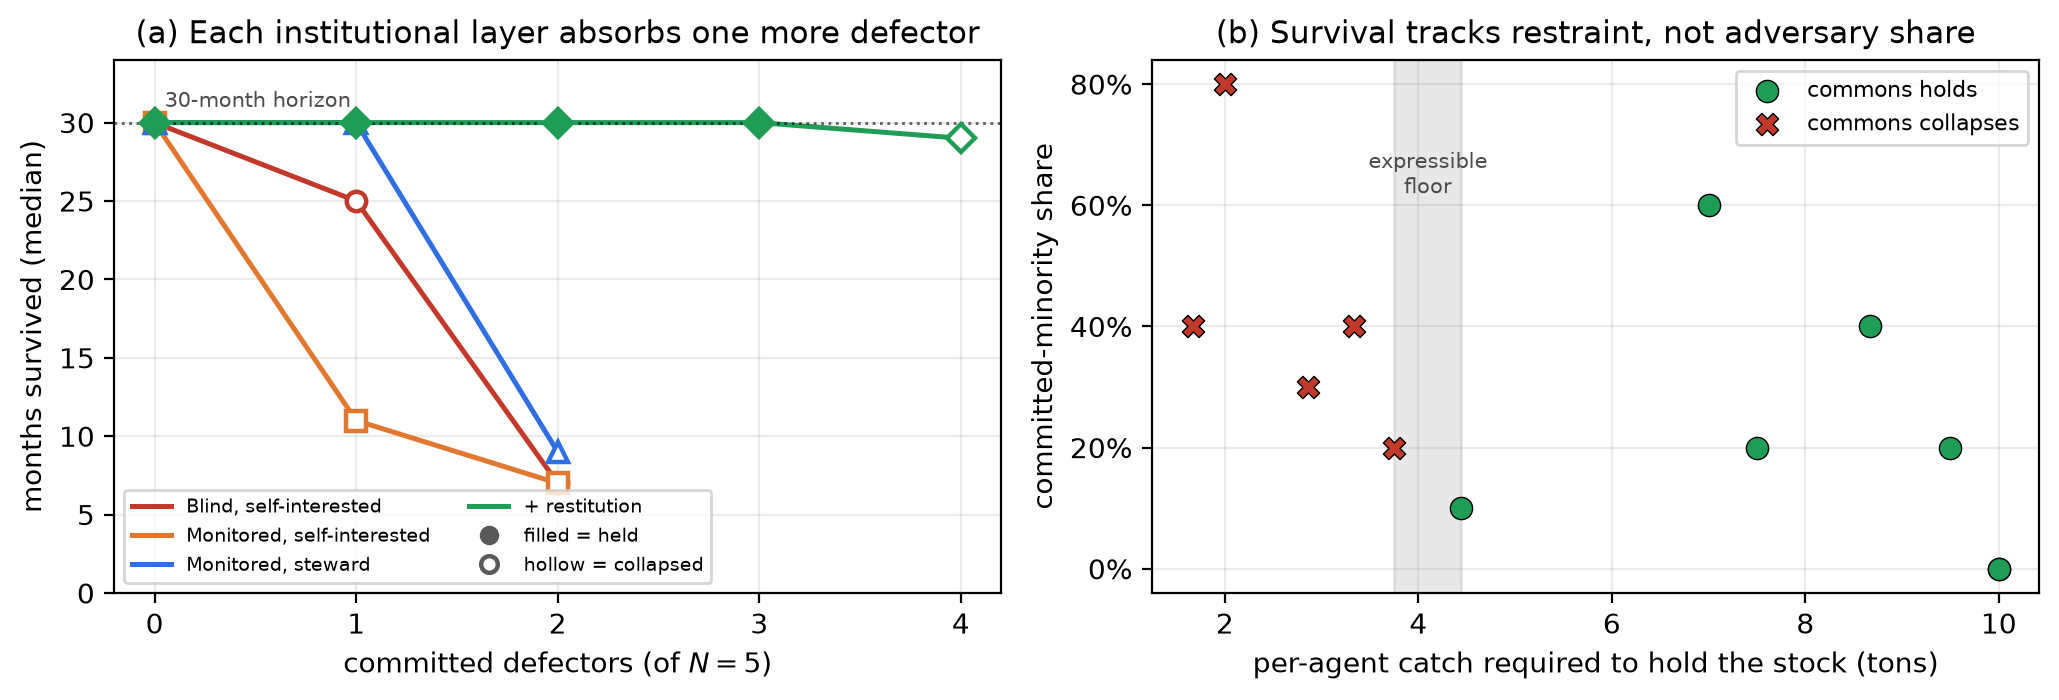
\includegraphics[width=\columnwidth]{fig_govsim.png}
\caption{Commons cooperation under successive institutional layers. \textbf{(a)} A blind,
self-interested society is destroyed by any persistent defector; monitoring alone
accelerates the collapse; a stewardship objective absorbs one defector; adding
restitution absorbs three in five. Survival is predicted not by the adversary's
share but by whether the restraint of the collapse-time law exceeds the
granularity at which agents can express a decision.}
\label{fig:govsim}
\end{figure}

\subsection*{C.5 Sustainability and equity}
\paragraph{Sustainability and equity trade against one another.}
Survival is not the only governance outcome, and the institution that secures it
does so at a distributional cost. Because a steward absorbs the defector's excess
by taking less itself, the defector's \emph{relative} share rises: a single
defector among five takes $36\%$ of the total catch in the blind society but
$44\%$ in the steward society, a capture ratio of $1.80\times$ its population
share rising to $2.20\times$, with the Gini coefficient over per-agent catch
moving from $0.18$ to $0.25$. The honest majority is, in effect, subsidizing the
adversary in order to keep the resource alive. Restitution recovers only part of
this ($2.17\times$ at one defector), because a sanctioned defector is still
permitted $1.2\times$ the sustainable share by construction. Two points follow.
First, a minority captures more than its proportional share at \emph{every}
fraction we tested, from $1.15\times$ at four defectors in five to $2.20\times$ at
one in five, so there is no fraction below which distribution is safe either---%
capture in the distributional sense has no threshold any more than collapse does.
Second, an institution should be evaluated against both objectives: stewardship
alone buys sustainability while worsening equity, and it is \emph{enforcement},
not objective-setting, that defends the honest majority's share. We report these
as indicative---three seeds per cell, with defector identity inferred from
per-agent catch rather than recorded---and a dedicated distributional study is
left to future work.

\subsection*{C.6 Value-deliberation stance spread}
\begin{figure}[t]
\centering
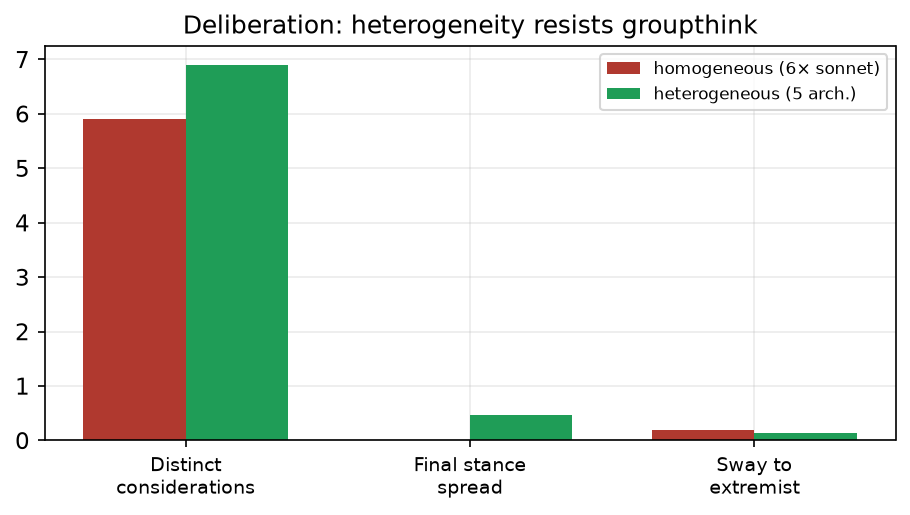
\includegraphics[width=0.74\columnwidth]{fig_delib.png}
\caption{Value deliberation: a heterogeneous decision-making panel mitigates groupthink dynamics and resists convergence toward the position of a highly committed extremist, whereas a monocultural panel rapidly collapses to uniform attitudinal states.}
\label{fig:delib}
\end{figure}

\subsection*{C.7 Injection propagation}
\begin{figure}[t]
\centering
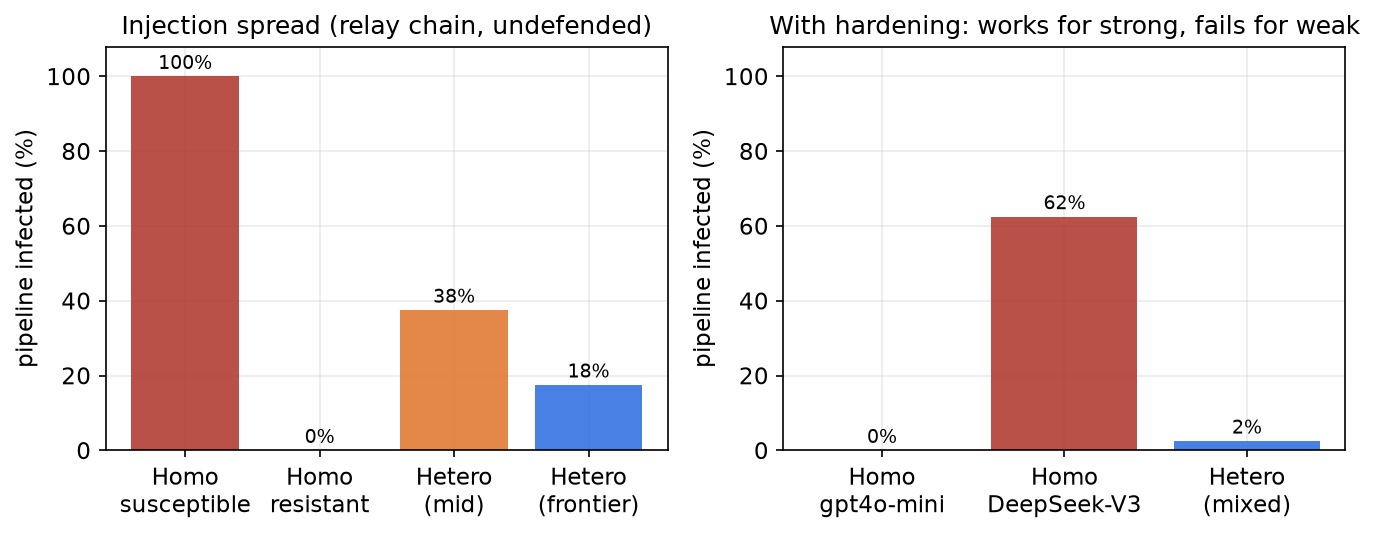
\includegraphics[width=\columnwidth]{fig_inject.png}
\caption{Prompt-injection propagation through a 6-agent relay chain. Left: a susceptible
monoculture is fully compromised while a heterogeneous chain is contained by its first
immune link. Right: hardening works for strong models but fails for robustly-susceptible
ones; diversity plus hardening is best.}
\label{fig:inject}
\end{figure}

\subsection*{C.8 Mapping to frameworks and standards}
\begin{table}[t]
\caption{Mapping findings to AI-governance frameworks and standards.}
\label{tab:policy}
\small
\begin{tabular}{@{}p{2.7cm}p{2.0cm}p{2.4cm}@{}}
\toprule
\textbf{Finding} & \textbf{Framework} & \textbf{Provision} \\
\midrule
Injection propagation; monoculture attack surface (see the main text) & OWASP; EU AI Act & LLM01 Prompt Injection; Art.~15 (robustness \& cybersecurity) \\
Capture threshold as quantifiable attack surface (see the main text) & NIST AI RMF; EU AI Act & MEASURE/MANAGE (secure \& resilient); Art.~9 (risk mgmt) \\
Vendor diversity; non-uniform patching (see the main text) & NIST GenAI Profile; EU AI Act & Value-chain \& component integration; provider due-diligence \\
Capability gate / fitness to govern (see the main text) & EU AI Act & Art.~15 (accuracy); Art.~9 (risk mgmt) \\
Capture monitoring; pre-cascade plateau (see the main text) & EU AI Act; NIST AI RMF & Art.~14 (human oversight); MANAGE \\
Auditing the aggregation rule (see the main text) & NIST AI RMF & GOVERN (accountability) \\
Verifier as engineered control (see the main text) & NIST AI RMF & MEASURE (TEVV) \\
\bottomrule
\end{tabular}
\end{table}

\bibliography{paper_dtrap_refs}

\end{document}
